% Options for packages loaded elsewhere
% Options for packages loaded elsewhere
\PassOptionsToPackage{unicode}{hyperref}
\PassOptionsToPackage{hyphens}{url}
\PassOptionsToPackage{dvipsnames,svgnames,x11names}{xcolor}
%
\documentclass[
  letterpaper,
  DIV=11,
  numbers=noendperiod]{scrartcl}
\usepackage{xcolor}
\usepackage{amsmath,amssymb}
\setcounter{secnumdepth}{-\maxdimen} % remove section numbering
\usepackage{iftex}
\ifPDFTeX
  \usepackage[T1]{fontenc}
  \usepackage[utf8]{inputenc}
  \usepackage{textcomp} % provide euro and other symbols
\else % if luatex or xetex
  \usepackage{unicode-math} % this also loads fontspec
  \defaultfontfeatures{Scale=MatchLowercase}
  \defaultfontfeatures[\rmfamily]{Ligatures=TeX,Scale=1}
\fi
\usepackage{lmodern}
\ifPDFTeX\else
  % xetex/luatex font selection
\fi
% Use upquote if available, for straight quotes in verbatim environments
\IfFileExists{upquote.sty}{\usepackage{upquote}}{}
\IfFileExists{microtype.sty}{% use microtype if available
  \usepackage[]{microtype}
  \UseMicrotypeSet[protrusion]{basicmath} % disable protrusion for tt fonts
}{}
\makeatletter
\@ifundefined{KOMAClassName}{% if non-KOMA class
  \IfFileExists{parskip.sty}{%
    \usepackage{parskip}
  }{% else
    \setlength{\parindent}{0pt}
    \setlength{\parskip}{6pt plus 2pt minus 1pt}}
}{% if KOMA class
  \KOMAoptions{parskip=half}}
\makeatother
% Make \paragraph and \subparagraph free-standing
\makeatletter
\ifx\paragraph\undefined\else
  \let\oldparagraph\paragraph
  \renewcommand{\paragraph}{
    \@ifstar
      \xxxParagraphStar
      \xxxParagraphNoStar
  }
  \newcommand{\xxxParagraphStar}[1]{\oldparagraph*{#1}\mbox{}}
  \newcommand{\xxxParagraphNoStar}[1]{\oldparagraph{#1}\mbox{}}
\fi
\ifx\subparagraph\undefined\else
  \let\oldsubparagraph\subparagraph
  \renewcommand{\subparagraph}{
    \@ifstar
      \xxxSubParagraphStar
      \xxxSubParagraphNoStar
  }
  \newcommand{\xxxSubParagraphStar}[1]{\oldsubparagraph*{#1}\mbox{}}
  \newcommand{\xxxSubParagraphNoStar}[1]{\oldsubparagraph{#1}\mbox{}}
\fi
\makeatother

\usepackage{color}
\usepackage{fancyvrb}
\newcommand{\VerbBar}{|}
\newcommand{\VERB}{\Verb[commandchars=\\\{\}]}
\DefineVerbatimEnvironment{Highlighting}{Verbatim}{commandchars=\\\{\}}
% Add ',fontsize=\small' for more characters per line
\usepackage{framed}
\definecolor{shadecolor}{RGB}{241,243,245}
\newenvironment{Shaded}{\begin{snugshade}}{\end{snugshade}}
\newcommand{\AlertTok}[1]{\textcolor[rgb]{0.68,0.00,0.00}{#1}}
\newcommand{\AnnotationTok}[1]{\textcolor[rgb]{0.37,0.37,0.37}{#1}}
\newcommand{\AttributeTok}[1]{\textcolor[rgb]{0.40,0.45,0.13}{#1}}
\newcommand{\BaseNTok}[1]{\textcolor[rgb]{0.68,0.00,0.00}{#1}}
\newcommand{\BuiltInTok}[1]{\textcolor[rgb]{0.00,0.23,0.31}{#1}}
\newcommand{\CharTok}[1]{\textcolor[rgb]{0.13,0.47,0.30}{#1}}
\newcommand{\CommentTok}[1]{\textcolor[rgb]{0.37,0.37,0.37}{#1}}
\newcommand{\CommentVarTok}[1]{\textcolor[rgb]{0.37,0.37,0.37}{\textit{#1}}}
\newcommand{\ConstantTok}[1]{\textcolor[rgb]{0.56,0.35,0.01}{#1}}
\newcommand{\ControlFlowTok}[1]{\textcolor[rgb]{0.00,0.23,0.31}{\textbf{#1}}}
\newcommand{\DataTypeTok}[1]{\textcolor[rgb]{0.68,0.00,0.00}{#1}}
\newcommand{\DecValTok}[1]{\textcolor[rgb]{0.68,0.00,0.00}{#1}}
\newcommand{\DocumentationTok}[1]{\textcolor[rgb]{0.37,0.37,0.37}{\textit{#1}}}
\newcommand{\ErrorTok}[1]{\textcolor[rgb]{0.68,0.00,0.00}{#1}}
\newcommand{\ExtensionTok}[1]{\textcolor[rgb]{0.00,0.23,0.31}{#1}}
\newcommand{\FloatTok}[1]{\textcolor[rgb]{0.68,0.00,0.00}{#1}}
\newcommand{\FunctionTok}[1]{\textcolor[rgb]{0.28,0.35,0.67}{#1}}
\newcommand{\ImportTok}[1]{\textcolor[rgb]{0.00,0.46,0.62}{#1}}
\newcommand{\InformationTok}[1]{\textcolor[rgb]{0.37,0.37,0.37}{#1}}
\newcommand{\KeywordTok}[1]{\textcolor[rgb]{0.00,0.23,0.31}{\textbf{#1}}}
\newcommand{\NormalTok}[1]{\textcolor[rgb]{0.00,0.23,0.31}{#1}}
\newcommand{\OperatorTok}[1]{\textcolor[rgb]{0.37,0.37,0.37}{#1}}
\newcommand{\OtherTok}[1]{\textcolor[rgb]{0.00,0.23,0.31}{#1}}
\newcommand{\PreprocessorTok}[1]{\textcolor[rgb]{0.68,0.00,0.00}{#1}}
\newcommand{\RegionMarkerTok}[1]{\textcolor[rgb]{0.00,0.23,0.31}{#1}}
\newcommand{\SpecialCharTok}[1]{\textcolor[rgb]{0.37,0.37,0.37}{#1}}
\newcommand{\SpecialStringTok}[1]{\textcolor[rgb]{0.13,0.47,0.30}{#1}}
\newcommand{\StringTok}[1]{\textcolor[rgb]{0.13,0.47,0.30}{#1}}
\newcommand{\VariableTok}[1]{\textcolor[rgb]{0.07,0.07,0.07}{#1}}
\newcommand{\VerbatimStringTok}[1]{\textcolor[rgb]{0.13,0.47,0.30}{#1}}
\newcommand{\WarningTok}[1]{\textcolor[rgb]{0.37,0.37,0.37}{\textit{#1}}}

\usepackage{longtable,booktabs,array}
\usepackage{calc} % for calculating minipage widths
% Correct order of tables after \paragraph or \subparagraph
\usepackage{etoolbox}
\makeatletter
\patchcmd\longtable{\par}{\if@noskipsec\mbox{}\fi\par}{}{}
\makeatother
% Allow footnotes in longtable head/foot
\IfFileExists{footnotehyper.sty}{\usepackage{footnotehyper}}{\usepackage{footnote}}
\makesavenoteenv{longtable}
\usepackage{graphicx}
\makeatletter
\newsavebox\pandoc@box
\newcommand*\pandocbounded[1]{% scales image to fit in text height/width
  \sbox\pandoc@box{#1}%
  \Gscale@div\@tempa{\textheight}{\dimexpr\ht\pandoc@box+\dp\pandoc@box\relax}%
  \Gscale@div\@tempb{\linewidth}{\wd\pandoc@box}%
  \ifdim\@tempb\p@<\@tempa\p@\let\@tempa\@tempb\fi% select the smaller of both
  \ifdim\@tempa\p@<\p@\scalebox{\@tempa}{\usebox\pandoc@box}%
  \else\usebox{\pandoc@box}%
  \fi%
}
% Set default figure placement to htbp
\def\fps@figure{htbp}
\makeatother





\setlength{\emergencystretch}{3em} % prevent overfull lines

\providecommand{\tightlist}{%
  \setlength{\itemsep}{0pt}\setlength{\parskip}{0pt}}



 


\KOMAoption{captions}{tableheading}
\makeatletter
\@ifpackageloaded{caption}{}{\usepackage{caption}}
\AtBeginDocument{%
\ifdefined\contentsname
  \renewcommand*\contentsname{Table of contents}
\else
  \newcommand\contentsname{Table of contents}
\fi
\ifdefined\listfigurename
  \renewcommand*\listfigurename{List of Figures}
\else
  \newcommand\listfigurename{List of Figures}
\fi
\ifdefined\listtablename
  \renewcommand*\listtablename{List of Tables}
\else
  \newcommand\listtablename{List of Tables}
\fi
\ifdefined\figurename
  \renewcommand*\figurename{Figure}
\else
  \newcommand\figurename{Figure}
\fi
\ifdefined\tablename
  \renewcommand*\tablename{Table}
\else
  \newcommand\tablename{Table}
\fi
}
\@ifpackageloaded{float}{}{\usepackage{float}}
\floatstyle{ruled}
\@ifundefined{c@chapter}{\newfloat{codelisting}{h}{lop}}{\newfloat{codelisting}{h}{lop}[chapter]}
\floatname{codelisting}{Listing}
\newcommand*\listoflistings{\listof{codelisting}{List of Listings}}
\makeatother
\makeatletter
\makeatother
\makeatletter
\@ifpackageloaded{caption}{}{\usepackage{caption}}
\@ifpackageloaded{subcaption}{}{\usepackage{subcaption}}
\makeatother
\usepackage{bookmark}
\IfFileExists{xurl.sty}{\usepackage{xurl}}{} % add URL line breaks if available
\urlstyle{same}
\hypersetup{
  pdftitle={Model},
  colorlinks=true,
  linkcolor={blue},
  filecolor={Maroon},
  citecolor={Blue},
  urlcolor={Blue},
  pdfcreator={LaTeX via pandoc}}


\title{Model}
\author{}
\date{}
\begin{document}
\maketitle


\begin{Shaded}
\begin{Highlighting}[]
\FunctionTok{library}\NormalTok{(tidyverse)}
\end{Highlighting}
\end{Shaded}

\begin{verbatim}
Warning: package 'tidyverse' was built under R version 4.4.3
\end{verbatim}

\begin{verbatim}
Warning: package 'ggplot2' was built under R version 4.4.3
\end{verbatim}

\begin{verbatim}
-- Attaching core tidyverse packages ------------------------ tidyverse 2.0.0 --
v dplyr     1.1.4     v readr     2.1.5
v forcats   1.0.0     v stringr   1.5.1
v ggplot2   4.0.0     v tibble    3.2.1
v lubridate 1.9.4     v tidyr     1.3.1
v purrr     1.0.2     
-- Conflicts ------------------------------------------ tidyverse_conflicts() --
x dplyr::filter() masks stats::filter()
x dplyr::lag()    masks stats::lag()
i Use the conflicted package (<http://conflicted.r-lib.org/>) to force all conflicts to become errors
\end{verbatim}

\begin{Shaded}
\begin{Highlighting}[]
\FunctionTok{library}\NormalTok{(spmodel)}
\end{Highlighting}
\end{Shaded}

\begin{verbatim}
Warning: package 'spmodel' was built under R version 4.4.3
\end{verbatim}

\subsection{Data}\label{data}

\begin{Shaded}
\begin{Highlighting}[]
\NormalTok{dat }\OtherTok{\textless{}{-}}\NormalTok{ vroom}\SpecialCharTok{::}\FunctionTok{vroom}\NormalTok{(}\StringTok{"PotatoCWSI.csv"}\NormalTok{) }\SpecialCharTok{\%\textgreater{}\%} \FunctionTok{filter}\NormalTok{(}\SpecialCharTok{!}\FunctionTok{is.na}\NormalTok{(CWSI))}
\end{Highlighting}
\end{Shaded}

\begin{verbatim}
Rows: 3889 Columns: 8
-- Column specification --------------------------------------------------------
Delimiter: ","
dbl (8): POINT_X, POINT_Y, SLOPE, TWI, ASPECT, ECA_SHALLOW, NDVI, CWSI

i Use `spec()` to retrieve the full column specification for this data.
i Specify the column types or set `show_col_types = FALSE` to quiet this message.
\end{verbatim}

\subsection{EDA}\label{eda}

\begin{Shaded}
\begin{Highlighting}[]
\FunctionTok{library}\NormalTok{(viridis)}
\end{Highlighting}
\end{Shaded}

\begin{verbatim}
Warning: package 'viridis' was built under R version 4.4.3
\end{verbatim}

\begin{verbatim}
Loading required package: viridisLite
\end{verbatim}

\begin{Shaded}
\begin{Highlighting}[]
\CommentTok{\# us\_states \textless{}{-} map\_data("state")}
\FunctionTok{ggplot}\NormalTok{() }\SpecialCharTok{+}
  \FunctionTok{geom\_point}\NormalTok{(}\AttributeTok{data =}\NormalTok{ dat, }\FunctionTok{aes}\NormalTok{(}\AttributeTok{x =}\NormalTok{ POINT\_X, }\AttributeTok{y =}\NormalTok{ POINT\_Y, }\AttributeTok{color =}\NormalTok{ CWSI))}\SpecialCharTok{+}
  \FunctionTok{scale\_color\_viridis}\NormalTok{()}
\end{Highlighting}
\end{Shaded}

\pandocbounded{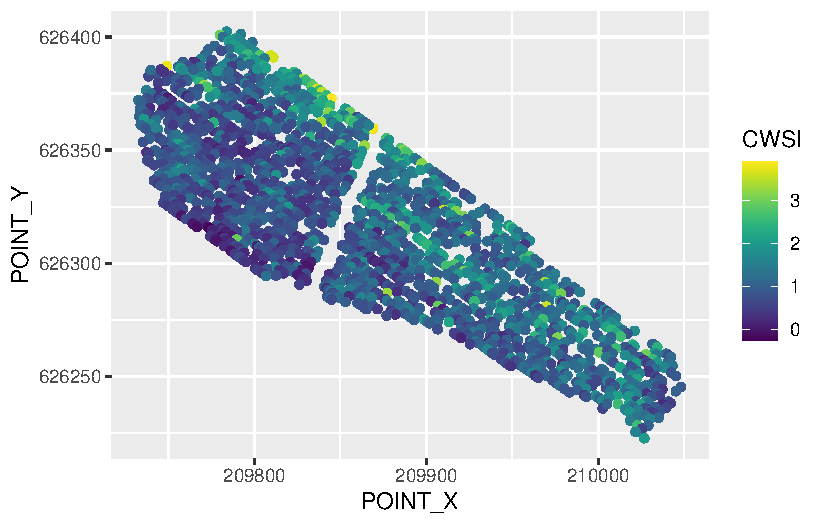
\includegraphics[keepaspectratio]{EDAandModel_files/figure-pdf/unnamed-chunk-3-1.pdf}}

make centers

\begin{Shaded}
\begin{Highlighting}[]
\NormalTok{K }\OtherTok{\textless{}{-}} \DecValTok{20}
\NormalTok{obs\_loc\_mat }\OtherTok{\textless{}{-}}\NormalTok{ dat[,}\FunctionTok{c}\NormalTok{(}\StringTok{"POINT\_X"}\NormalTok{, }\StringTok{"POINT\_Y"}\NormalTok{)]}

\NormalTok{centers }\OtherTok{\textless{}{-}}\NormalTok{ fields}\SpecialCharTok{::}\FunctionTok{cover.design}\NormalTok{(obs\_loc\_mat, }\AttributeTok{nd =}\NormalTok{ K)}\SpecialCharTok{$}\NormalTok{design}
\end{Highlighting}
\end{Shaded}

\begin{Shaded}
\begin{Highlighting}[]
\NormalTok{dist\_btwn\_centers }\OtherTok{\textless{}{-}}\NormalTok{ fields}\SpecialCharTok{::}\FunctionTok{rdist}\NormalTok{(centers)}

\NormalTok{the\_scale }\OtherTok{\textless{}{-}} \FloatTok{1.5}\SpecialCharTok{*}\FunctionTok{max}\NormalTok{(}\FunctionTok{apply}\NormalTok{(dist\_btwn\_centers, }\DecValTok{1}\NormalTok{, }\ControlFlowTok{function}\NormalTok{(x)\{}\FunctionTok{sort}\NormalTok{(x)\}[}\DecValTok{2}\NormalTok{]))}
\end{Highlighting}
\end{Shaded}

\begin{Shaded}
\begin{Highlighting}[]
\FunctionTok{library}\NormalTok{(FRK)}
\end{Highlighting}
\end{Shaded}

\begin{verbatim}
Warning: package 'FRK' was built under R version 4.4.3
\end{verbatim}

\begin{verbatim}

Attaching package: 'FRK'
\end{verbatim}

\begin{verbatim}
The following object is masked from 'package:stats':

    simulate
\end{verbatim}

\begin{Shaded}
\begin{Highlighting}[]
\NormalTok{spat\_features }\OtherTok{\textless{}{-}} \FunctionTok{local\_basis}\NormalTok{(}
  \AttributeTok{manifold =} \FunctionTok{plane}\NormalTok{(),}
  \AttributeTok{loc =}\NormalTok{ centers,}
  \AttributeTok{scale =} \FunctionTok{rep}\NormalTok{(the\_scale,K),}
  \AttributeTok{type =} \StringTok{"bisquare"}
\NormalTok{) }\SpecialCharTok{\%\textgreater{}\%}
  \FunctionTok{eval\_basis}\NormalTok{(}\FunctionTok{as.matrix}\NormalTok{(obs\_loc\_mat)) }\SpecialCharTok{\%\textgreater{}\%}
  \FunctionTok{as.matrix}\NormalTok{()}

\FunctionTok{colnames}\NormalTok{(spat\_features) }\OtherTok{\textless{}{-}} \FunctionTok{paste0}\NormalTok{(}\StringTok{"SF"}\NormalTok{, }\DecValTok{1}\SpecialCharTok{:}\NormalTok{K)}
\end{Highlighting}
\end{Shaded}

\begin{Shaded}
\begin{Highlighting}[]
\NormalTok{spatial\_dataframe }\OtherTok{\textless{}{-}} \FunctionTok{bind\_cols}\NormalTok{(dat, spat\_features)}
\end{Highlighting}
\end{Shaded}

\begin{Shaded}
\begin{Highlighting}[]
\NormalTok{spat\_lm }\OtherTok{\textless{}{-}} \FunctionTok{lm}\NormalTok{(CWSI }\SpecialCharTok{\textasciitilde{}}\NormalTok{ . }\SpecialCharTok{{-}}\NormalTok{POINT\_X }\SpecialCharTok{{-}}\NormalTok{ POINT\_Y, }\AttributeTok{data =}\NormalTok{ spatial\_dataframe)}
\CommentTok{\#summary(spat\_lm)}

\NormalTok{spat\_inter }\OtherTok{\textless{}{-}} \FunctionTok{lm}\NormalTok{(CWSI }\SpecialCharTok{\textasciitilde{}}\NormalTok{ . }\SpecialCharTok{{-}}\NormalTok{POINT\_X }\SpecialCharTok{{-}}\NormalTok{ POINT\_Y }\SpecialCharTok{+}\NormalTok{ TWI}\SpecialCharTok{:}\NormalTok{ECA\_SHALLOW }\SpecialCharTok{+}\NormalTok{ ASPECT}\SpecialCharTok{:}\NormalTok{SLOPE, }\AttributeTok{data =}\NormalTok{ spatial\_dataframe)}
\CommentTok{\#summary(spat\_inter)}
\FunctionTok{anova}\NormalTok{(spat\_lm, spat\_inter)}
\end{Highlighting}
\end{Shaded}

\begin{verbatim}
Analysis of Variance Table

Model 1: CWSI ~ (POINT_X + POINT_Y + SLOPE + TWI + ASPECT + ECA_SHALLOW + 
    NDVI + SF1 + SF2 + SF3 + SF4 + SF5 + SF6 + SF7 + SF8 + SF9 + 
    SF10 + SF11 + SF12 + SF13 + SF14 + SF15 + SF16 + SF17 + SF18 + 
    SF19 + SF20) - POINT_X - POINT_Y
Model 2: CWSI ~ (POINT_X + POINT_Y + SLOPE + TWI + ASPECT + ECA_SHALLOW + 
    NDVI + SF1 + SF2 + SF3 + SF4 + SF5 + SF6 + SF7 + SF8 + SF9 + 
    SF10 + SF11 + SF12 + SF13 + SF14 + SF15 + SF16 + SF17 + SF18 + 
    SF19 + SF20) - POINT_X - POINT_Y + TWI:ECA_SHALLOW + ASPECT:SLOPE
  Res.Df    RSS Df Sum of Sq      F    Pr(>F)    
1   1917 326.67                                  
2   1915 319.57  2     7.095 21.258 7.393e-10 ***
---
Signif. codes:  0 '***' 0.001 '**' 0.01 '*' 0.05 '.' 0.1 ' ' 1
\end{verbatim}

\begin{Shaded}
\begin{Highlighting}[]
\CommentTok{\#spat\_lm}


\NormalTok{spatial\_dataframe}\SpecialCharTok{$}\NormalTok{resids }\OtherTok{\textless{}{-}} \FunctionTok{residuals}\NormalTok{(spat\_inter)}

\FunctionTok{plot}\NormalTok{(spmodel}\SpecialCharTok{::}\FunctionTok{esv}\NormalTok{(resids }\SpecialCharTok{\textasciitilde{}} \DecValTok{1}\NormalTok{, }\AttributeTok{data =}\NormalTok{ spatial\_dataframe, }\AttributeTok{xcoord =}\NormalTok{ POINT\_X, }\AttributeTok{ycoord =}\NormalTok{ POINT\_Y))}
\end{Highlighting}
\end{Shaded}

\pandocbounded{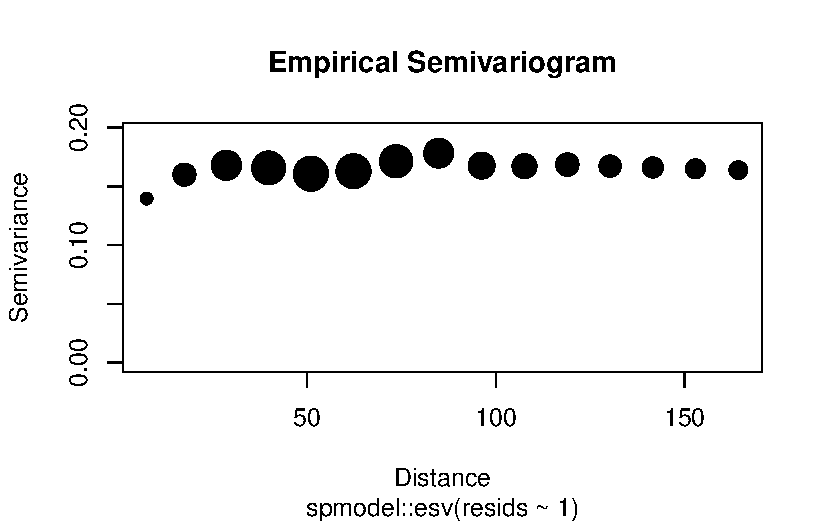
\includegraphics[keepaspectratio]{EDAandModel_files/figure-pdf/unnamed-chunk-9-1.pdf}}

Normal

\begin{Shaded}
\begin{Highlighting}[]
\NormalTok{stand\_resids }\OtherTok{\textless{}{-}}\NormalTok{ (spatial\_dataframe}\SpecialCharTok{$}\NormalTok{resids }\SpecialCharTok{{-}} \FunctionTok{mean}\NormalTok{(spatial\_dataframe}\SpecialCharTok{$}\NormalTok{resids))}\SpecialCharTok{/}\FunctionTok{sd}\NormalTok{(spatial\_dataframe}\SpecialCharTok{$}\NormalTok{resids)}

\FunctionTok{shapiro.test}\NormalTok{(stand\_resids)}
\end{Highlighting}
\end{Shaded}

\begin{verbatim}

    Shapiro-Wilk normality test

data:  stand_resids
W = 0.98048, p-value = 1.21e-15
\end{verbatim}

\begin{Shaded}
\begin{Highlighting}[]
\FunctionTok{hist}\NormalTok{(stand\_resids, }\AttributeTok{freq =}\NormalTok{ F)}
\FunctionTok{curve}\NormalTok{(}\FunctionTok{dnorm}\NormalTok{(x), }\AttributeTok{add =}\NormalTok{ T)}
\end{Highlighting}
\end{Shaded}

\pandocbounded{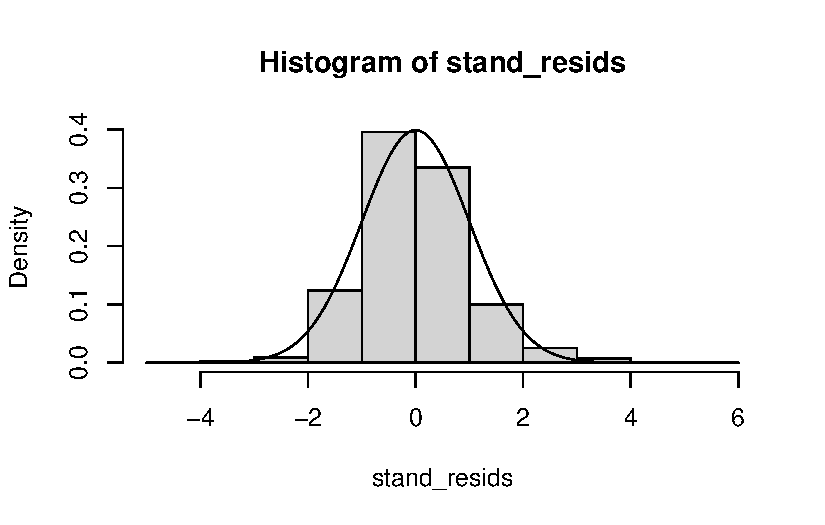
\includegraphics[keepaspectratio]{EDAandModel_files/figure-pdf/unnamed-chunk-10-1.pdf}}

Equal Var

\begin{Shaded}
\begin{Highlighting}[]
\NormalTok{fitteds }\OtherTok{\textless{}{-}} \FunctionTok{fitted}\NormalTok{(spat\_lm)}
\FunctionTok{plot}\NormalTok{(fitteds, stand\_resids)}
\end{Highlighting}
\end{Shaded}

\pandocbounded{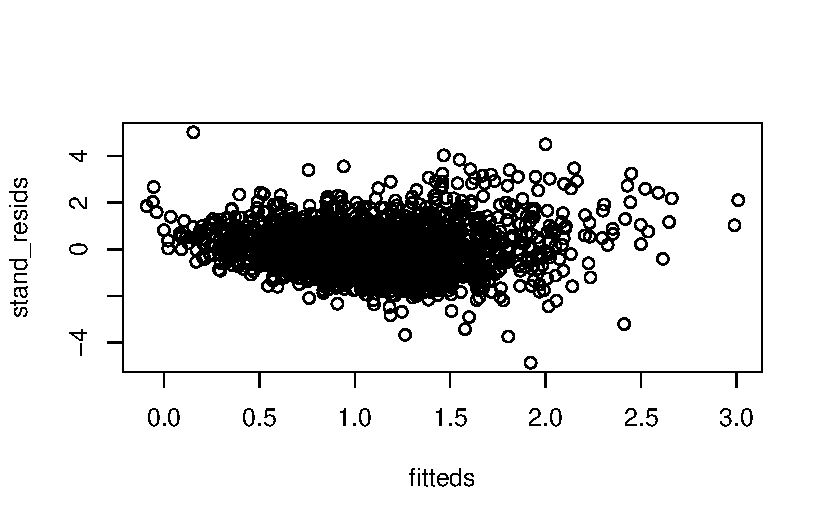
\includegraphics[keepaspectratio]{EDAandModel_files/figure-pdf/unnamed-chunk-11-1.pdf}}

\begin{Shaded}
\begin{Highlighting}[]
\NormalTok{lmtest}\SpecialCharTok{::}\FunctionTok{bptest}\NormalTok{(spat\_lm)}
\end{Highlighting}
\end{Shaded}

\begin{verbatim}

    studentized Breusch-Pagan test

data:  spat_lm
BP = 216.11, df = 25, p-value < 2.2e-16
\end{verbatim}

R squared

\begin{Shaded}
\begin{Highlighting}[]
\NormalTok{r2 }\OtherTok{\textless{}{-}} \FunctionTok{cor}\NormalTok{(}\FunctionTok{fitted}\NormalTok{(spat\_inter), spatial\_dataframe}\SpecialCharTok{$}\NormalTok{CWSI)}\SpecialCharTok{\^{}}\DecValTok{2} 
\NormalTok{r2}
\end{Highlighting}
\end{Shaded}

\begin{verbatim}
[1] 0.5440203
\end{verbatim}

\begin{Shaded}
\begin{Highlighting}[]
\NormalTok{spatial\_dataframe}\SpecialCharTok{$}\NormalTok{resids }\OtherTok{\textless{}{-}} \ConstantTok{NULL}
\end{Highlighting}
\end{Shaded}





\end{document}
